\documentclass{article}
\usepackage[utf8]{inputenc}
\usepackage{float}
\usepackage{graphicx}
\usepackage{multirow} % Add multirows for tables
\usepackage{subcaption}

\title{A multi-output state space model}
\author{Sergio Garrido}

\begin{document}
\maketitle

\section{Motivation}
The main motivation for this model is the use of predicted activities in an activity-based model of transportation. The aims of these models are to predict transport demand based on daily activities of people. For the purpose of this project, we are only interested in predicting the last activity, mode choice and location of a person. We managed to do predictions for the activities and the mode choice but not for the locations. A second choice that was made was the modeling choice. A state space model makes sense (of course this can be debated) from a theoretical perspective. Realization of choices of people depend on previous plans, these plans are represented by each of the hidden states and at the same time, these plans are affected by both exogenous variables such as the time of the day or the day of the week, and the plan from the last period ,i.e., the previous hidden state. 

\section{Data analysis and pre processing}

We have two data sets which (actually) belong to a same survey: TU data set. The TU data set is a trip survey conducted in Denmark and contains information on trips of people and some socio-economic variables. We are going to use the "Sessions.csv" data set and the the "Tur.csv" data set. The first contains the socio-economic data of the interviewees such as income, number of members in the family, municipality of origin, etc. The latter contains a travel diary for a day of this individual. The travel diary contains all the trips taken by this person on a day, when did the person made the trip, what was the purpose of it, what was the mode choice, etc.

Even though we didn't use the socio-economic variables in this project, if needed be the case, they would be selected based on "economics" intuition. This means, what are the drivers of choices of people. Some of these variables (although not an exhaustive list) are: income, municipality of residency, main occupation, etc. For the purpose of this project we only used temporal information as stated above. And interesting alley of research would be to use also socio-economic variables. 

Data pre processing was relatively easy. A random sample of 0.5\% of the observations was taken from the data set. Individuals with missing values were dropped. The outcome variables were reduced in dimensionality to a dimensionality of 5 (each). 

\section{Model}
\subsection{Model framework}

The final model for this project is a state space model using the spatio-temporal variables to affect each hidden state. The length of the total number of hidden states is dynamic: we have a different length for each person. The hidden state and some infered parameters predict both the activity of the person and the mode choice. The intercept for each of the activities and mode choices is inferred for *each* observation. For more clarity, the data generation process is the following:

\subsection{Data Generating process}

\begin{enumerate}
    \item Draw global parameters from hidden state to hidden state $\beta_{hs, hs} \sim \mathcal{N}(\beta_{hs, hs} | \textbf{0}, \, 5)$
    \item Draw global parameters on the variance-covariance matrix $\tau \sim \mathcal{Cauchy_{+}}(\tau | \textbf{0}, \, 5)$
    \item Draw global parameters from hidden state to activity     $\beta_{hs, a} \sim \mathcal{N}(\beta_{hs, a} | \textbf{0}, \, 5)$
    \item Draw global parameters from hidden state to mode choice  $\beta_{hs, mc} \sim \mathcal{N}(\beta_{hs, mc} | \textbf{0}, \, 5)$
    \item For each choice ($ca$) in activities:
    \begin{enumerate}
        \item Draw $\mu_{ca} \sim \mathcal{N}(\mu_{ca} | \textbf{0}, \, 5)$  The mean hyper-prior
        \item Draw $\sigma_{ca} \sim \mathcal{Cauchy_{+}}(\sigma_{ca} | \textbf{0}, \, 5)$ The variance hyper-prior
    \end{enumerate}
    \item For each choice ($cmc$) in mode choice:
    \begin{enumerate}
        \item Draw $\mu_{cmc} \sim \mathcal{N}(\mu_{cmc} | \textbf{0}, \, 5)$  The mean hyper-prior
        \item Draw $\sigma_{cmc} \sim Cauchy_{+}(\sigma_{cmc} | \textbf{0}, \, 5)$  The variance hyper-prior
    \end{enumerate}
    \item For each individual ($i$):
    \begin{enumerate}
        \item Draw the initial hidden state: $hs_{0} \sim \mathcal{N}(hs_{0} | \textbf{0}, \, \Sigma)$
        \item For each choice ($ca$) in activities:
        \begin{enumerate}
            \item Draw the intercept: $\alpha_{i, ca} \sim \mathcal{N}(\alpha_{i, ca} | \mu_{ca}, \, \sigma_{ca})$
        \end{enumerate}
        \item For each choice ($cmc$) in mode choice:
        \begin{enumerate}
            \item Draw the intercept: $\alpha_{i, cmc} \sim \mathcal{N}(\alpha_{i, cmc} | \mu_{cmc}, \, \sigma_{cmc})$
        \end{enumerate}
        \item For each time ($t$) in the observation's number of periods $T_{i}$:
        \begin{enumerate}
            \item $Activity_{t} \sim CategoricalLogit(\beta_{hs, a}*hs_{t}+\alpha_{i, a})$
            \item $ModeChoice_{t} CategoricalLogit(\beta_{hs, mc}*hs_{t}+\alpha_{i, mc})$
            \item if $t \neq T_{n}$:
            \begin{enumerate}
                \item $hs_{t+1} \sim \mathcal{N}(hs_{t+1} | \beta_{hs, hs}*hs_{t}, \, \Sigma)$
            \end{enumerate}
        \end{enumerate}
    \end{enumerate}
\end{enumerate}

\subsection{Graphical representation}

\begin{figure}[htp!]
    \centering
    \begin{subfigure}[b]{\textwidth}
        \includegraphics[width=.9\textwidth]{assets/model_representation.png}
    \end{subfigure}
    \caption{Graphical model}
    \label{fig:graphical_model}
\end{figure}

\section{Results}

The model was evaluated using the accuracy of the prediction of the last activity. The hierarchical model performs considerably better than the rest of the models. The models which don't use the hierarchical intercept, overfit to those choices which are most common in the data set.

A second interesting result is the distribution of the hyper-parameters. Initially, I infered the parameters of the model using variational inference which is considerably faster than monte carlo methods, however, in the last model I also wanted to study potential multimodality in the estimated parameters since I suspected they would have more than one mode. It was not a big surprise that most(8-9) of all (10, 5 for means and 5 for variances) of the hyperpriors for the activity choice had two modes. This graphs can be found at the end of the notebook. 

\begin{figure}[H]
    \centering
    \begin{subfigure}[b]{\textwidth}
        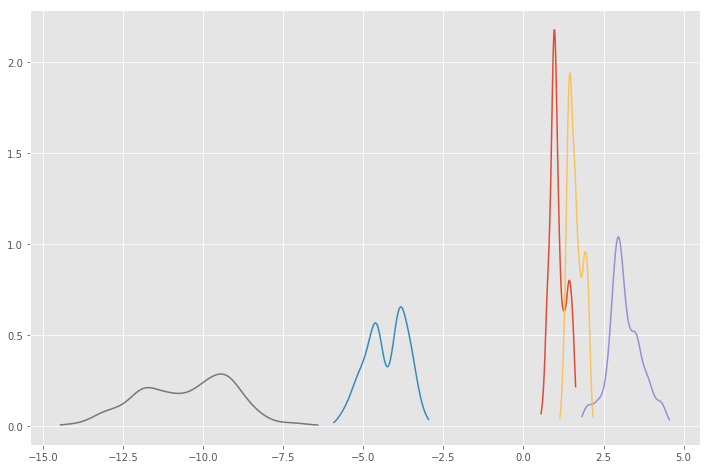
\includegraphics[width=.45\textwidth]{assets/hp_mu.png}\hfill
        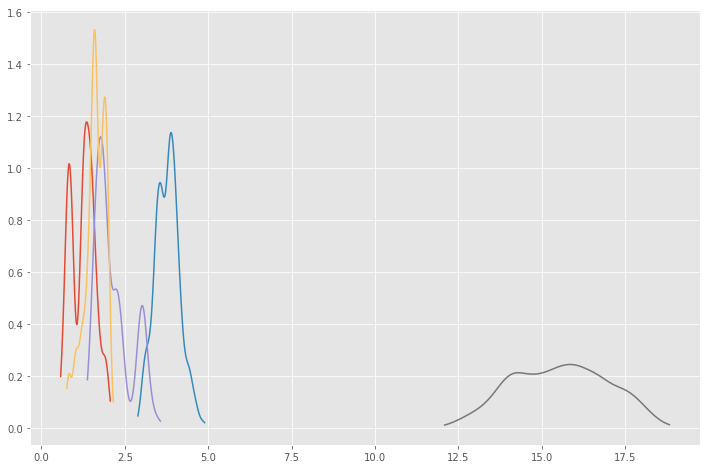
\includegraphics[width=.45\textwidth]{assets/hp_sigma.png}\hfill
    \end{subfigure}
    \caption{hyper-prior distributions for the mean (left) and variance (right) of the intercept for the activities}
    \label{fig:hp}
\end{figure}

A third and final interesting result is the distribution of the last hidden state of the observations. In the final model, I used a hidden state of dimensionality 2 which allowed me to plot one as a function of the other (although if they had higher dimensions we would just use a dimensionality reduction algorithm like t-sne or MDS algorithms). The initial state is as we would expect, it is normally distributed with some correlation between the two states. The really interesting one is the last state which has two clear modes, one that looks like a normal with a strong positive correlation and a second mode which looks like a horseshoe. When I graph this, distinguishing which of them correspond to which activity, they seem to (slightly) separate the type of the activities by the position in the 2d map. However, for the mode choice case, they don't seem to separate anything. 

\begin{figure}[H]
    \centering
    \begin{subfigure}[b]{\textwidth}
        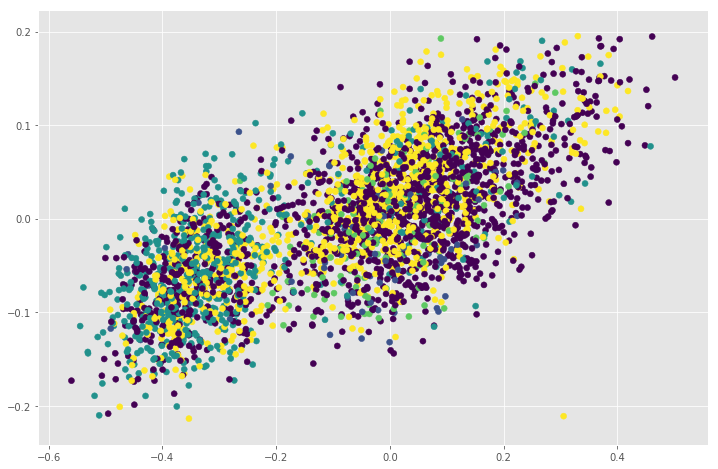
\includegraphics[width=.45\textwidth]{assets/first_hs.png}\hfill
        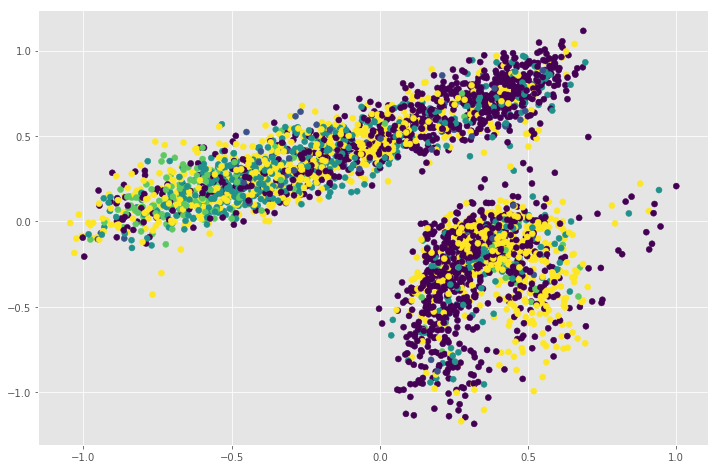
\includegraphics[width=.45\textwidth]{assets/last_hs.png}\hfill
    \end{subfigure}
    \caption{Distribution of the 2D hidden states. The right figure corresponds to the first hidden state and the left figure corresponds to the last hidden state. The colors correspond to the activities these hidden states represented}
    \label{fig:hs}
\end{figure}

\section{Extensions}

Some interesting directions in which I can take this model are:
\begin{itemize}
    \item Adding the rest of the variables of interest, meaning the location and potentially the dwelling time
    \item Further exploration of the hidden-state which seems to be capturing some feature of the data set which is not exactly the activity or the mode choice
    \item The use of socio-economic variables affecting something in the model (it is uncertain to me as they are fixed for all the periods). Probably the hyper-priors
    \item The implementation of non-linearities on the relations between variables and hidden-state and/or hidden state and hidden state
    \item The implementation of missing values imputation
    \item The modeling of whole sequences as opposed to only only element of the sequence. This can be done by modeling the number of journeys of a person as a Poisson distribution
    \item The understanding of causality, counterfactuals and interventions in a final model
\end{itemize}

\end{document}
